\begin{figure}[H]
    \begin{subfigure}[t]{.3\textwidth}
        \caption{}
        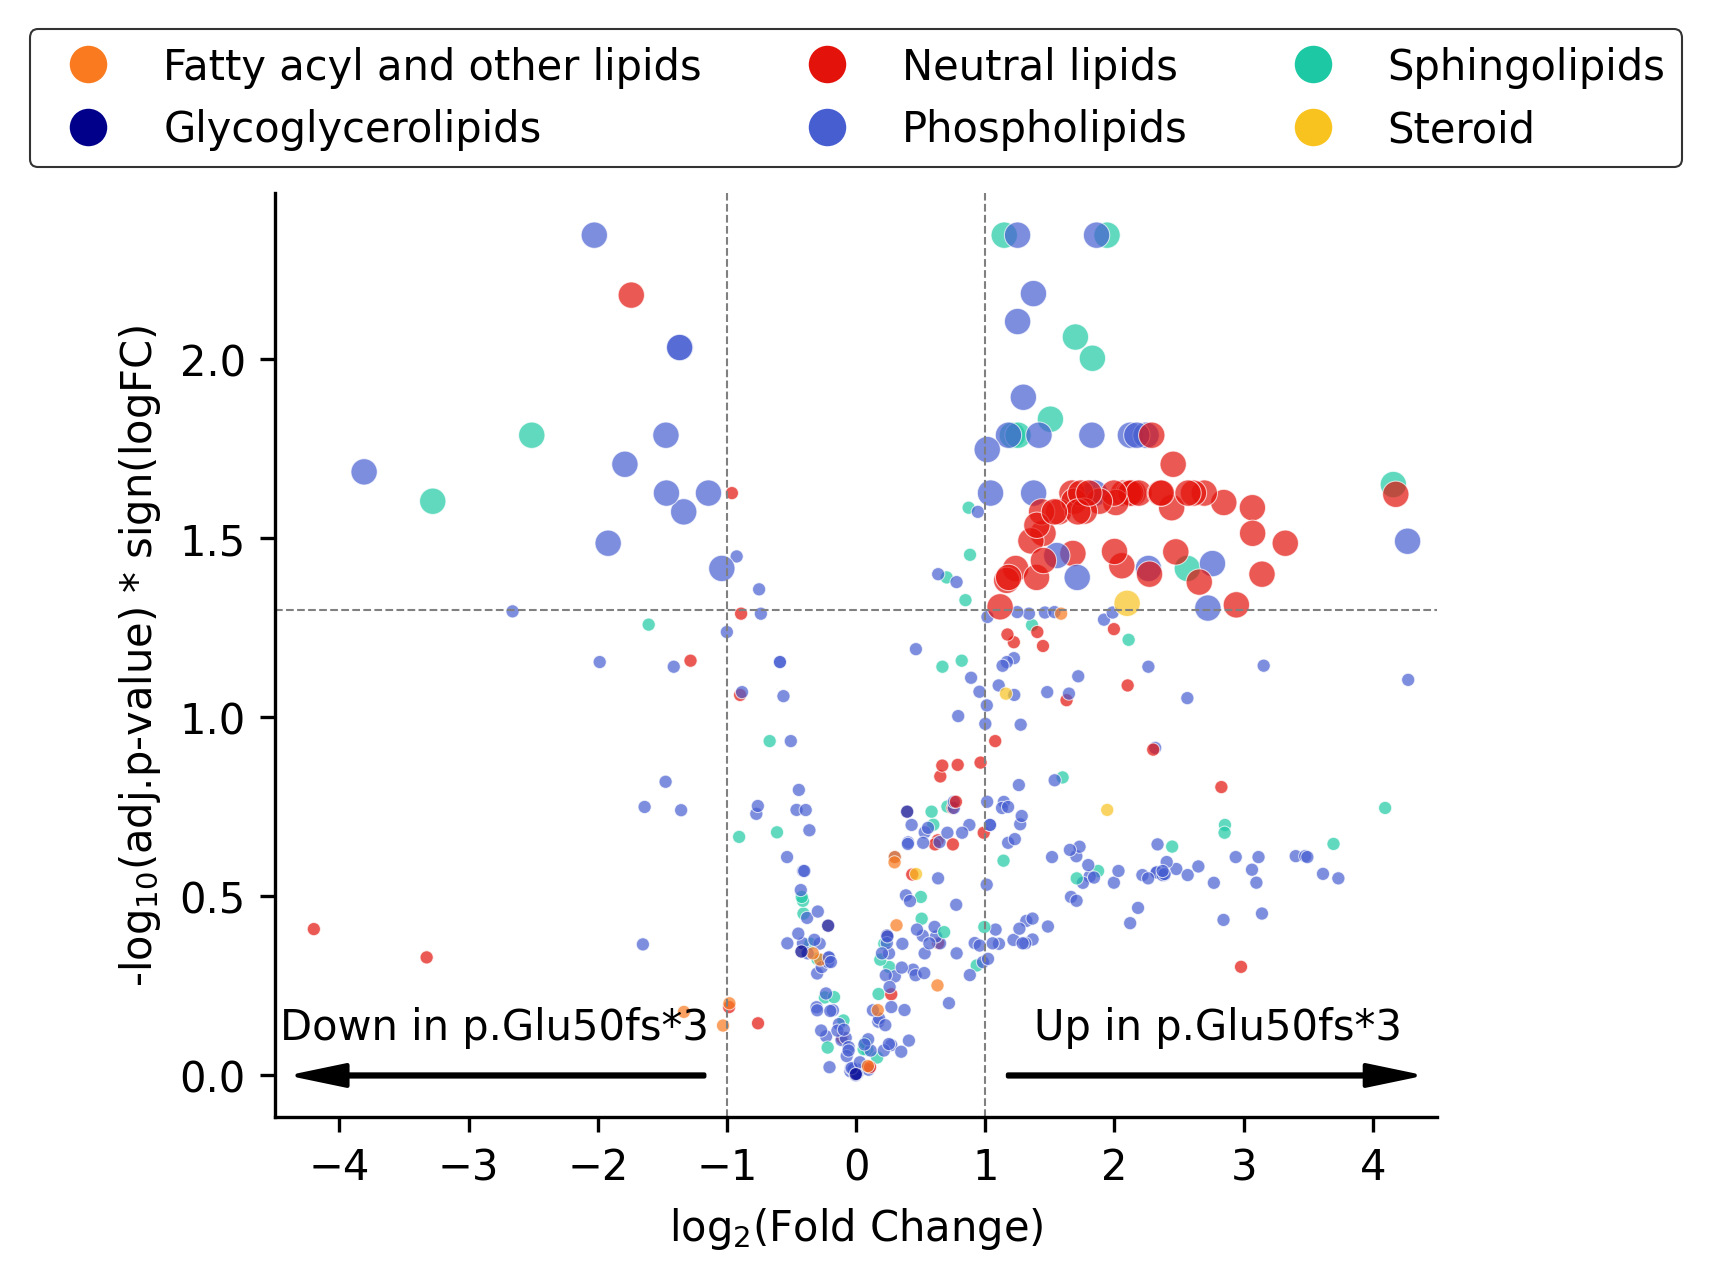
\includegraphics[width=\textwidth]{./main_plots/iN_lipids_overview.png}        
    \end{subfigure} 
    \begin{subfigure}[t]{.3\textwidth}
        \caption{}
        \includegraphics[width=\textwidth]{./main_plots/lipids_table.png}        
    \end{subfigure} 
    \begin{subfigure}[t]{.3\textwidth}
        \caption{}
        \includegraphics[width=\textwidth]{./main_plots/tg_carbons.png}        
    \end{subfigure} 
    \begin{subfigure}[t]{.3\textwidth}
        \caption{}
        \includegraphics[width=\textwidth]{./main_plots/G2_PC_volcano_sat.png}        
    \end{subfigure} 
    \begin{subfigure}[t]{.3\textwidth}
        \caption{}
        \includegraphics[width=\textwidth]{./main_plots/G2_PC_volcano_unsat.png}        
    \end{subfigure} 
    \begin{subfigure}[t]{.3\textwidth}
        \caption{}
        \includegraphics[width=\textwidth]{./main_plots/pc_unsat.png}        
    \end{subfigure} 
    \begin{subfigure}[t]{.3\textwidth}
        \caption{}
        \includegraphics[width=\textwidth]{./main_plots/lipids_table_y622.png}        
    \end{subfigure}
    \begin{subfigure}[t]{.3\textwidth}
        \caption{}
        \includegraphics[width=\textwidth]{./main_plots/Y622_PC_volcano_sat.png}        
    \end{subfigure} 
    \begin{subfigure}[t]{.3\textwidth}
        \caption{}
        \includegraphics[width=\textwidth]{./main_plots/tg_carbons_y622.png}        
    \end{subfigure} 
    \begin{subfigure}[t]{.3\textwidth}
        \caption{}
        \includegraphics[width=\textwidth]{./main_plots/pc_unsat_y622.png}        
    \end{subfigure} 
    \begin{subfigure}[t]{.2\textwidth}
        \caption{}
        \includegraphics[width=\textwidth]{./extended_plots/g2_lpcat.png}        
    \end{subfigure} 
    \begin{subfigure}[t]{.2\textwidth}
        \caption{}
        \includegraphics[width=\textwidth]{./extended_plots/y622_lpcat.png}        
    \end{subfigure} 
    \caption{
        \textbf{LCMS-lipidomics in ABCA7 LoF iNs.}\\
    }
    \label{fig:main_lipids}
\end{figure}
\begin{itemize}
    \item[\textbf{(A)}] Volcano plot of significantly perturbed lipid species identified by LC-MS in p.Glu50fs*3 vs. WT iNs (BH FDR-adjusted $p<0.05$, $|\log_2(\text{FC})|>1$), colored by lipid class. $N=6$ wells per genotype.
    \item[\textbf{(B)}] Significantly perturbed lipid species from (A), summarized by lipid subclass.
    \item[\textbf{(C)}] Distribution of triglyceride fold changes grouped by fatty acid chain length and saturation.
    \item[\textbf{(D)}] Volcano plot highlighting significantly perturbed phosphatidylcholine species containing saturated or monounsaturated fatty acids (SFA/MUFA; BH FDR-adjusted $p<0.05$, $|\log_2(\text{FC})|>1$).
    \item[\textbf{(E)}] Volcano plot highlighting significantly perturbed phosphatidylcholine species containing polyunsaturated fatty acids (PUFA; BH FDR-adjusted $p<0.05$, $|\log_2(\text{FC})|>1$).
    \item[\textbf{(F)}] Distribution of phosphatidylcholine fold changes grouped by fatty acid chain length and saturation.
    \item[\textbf{(G)}] Table summarizing significantly perturbed lipid species by lipid subclass in p.Tyr622* vs. WT iNs ($N=10$ WT, $8$ p.Tyr622* wells; BH FDR-adjusted $p<0.05$, $|\log_2(\text{FC})|>1$).
    \item[\textbf{(H)}] Volcano plot showing lipid species from (G), colored by lipid class; phosphatidylcholines highlighted in blue.
    \item[\textbf{(I,J)}] Same analysis as (C,F), but comparing p.Tyr622* vs. WT iNs.
    \item[\textbf{(K,L)}] Expression changes (mRNA) of LPCAT genes comparing p.Tyr622* vs. WT and p.Glu50fs*3 vs. WT iNs.
\end{itemize}